\chapter{Operations on Graphs}

Rishnak caught up with Ajur who was walking with Jura. Rishnak started the session saying it was about various graph operations.
Ajur aksed whether they were similar to arithmetical operations (like addition, subtraction, multiplication) on numbers or set operations (such as union, intersection, complement). Rishnak said that there are a number of binary operations and since graphs are represented as sets, many of the operations were similar to set operations. Rishnak added that with Graph operations one can generate more graphs and one can also how graphs eveolve.

Rishnak listed the following binary graph operations:
\begin{enumerate}
    \item Graph Union: Union of two graphs $G_3=(V_3,E_3)$= $G_1=(V_1,E_1)$ and $G_2=(V_2,E_2)$ where $V_3= V_1 \cup V_2$ and
    $E_3=E_1\cup E_2$. Naturally this graph $G_3$ is not connected.
    \item Graph Complement: Complement of a Graph $H=(V_2,E_2)$ of $G=(V_1,E_1)$, where $V_2$ = $V_1$ and $E_2$=$\{e| e \notin E_1\}$ Please see Figures \ref{17g1} \ref{17g2}.
    \item Vertex Addition: Vertex Addition to a graph $G_1=V_1,E_1)$ is a graph $G_2=(V_2,E_2)$  where $V_2=V_1 \cup \{x| \notin V_1\}$ and $E_2=E_1 \cup \{(x,y)  |$ for some  $y  \in Y \subset~ of~ V_1\}$ Please see Figure \ref{17g3} of adding a vertex to \ref{17g1}. Barabassi - Albert used a version of this to generate graphs.\footnote {In Barabassi-Albert model the new vertex adds an edge to an existing vertex with a probability related to the degree of that vertex to generate graphs.}
    \item  The Cartesian product $G_1$ $ \square $  $G_2$ is a graph $G_3$ such that
the vertex set of $G_3$  is the Cartesian product $V(G_1) × V(G_2)$; and
two vertices $(u,u' )$ and $(v,v' )$ are adjacent in $G_3$ if and only if either
$u = v$ and $u'$ is adjacent to $v'$ in $G_2$, or
$u' = v'$ and $u$ is adjacent to $v$ in $G_1$. Please see Graphs in Figures \ref{17g4} \ref{17g5} and \ref{17g6}
\item Given a graph $G$, the line graph  of $G$ denoted by $L(G)$ is a graph such that
each vertex of $L(G)$ represents an edge of $G$; and
two vertices in $L(G)$ are adjacent the corresponding edges share a common end vertex. Please see Figures \ref{17g7} and \ref{17g8}
\end{enumerate}
\begin{figure}
\begin{center}
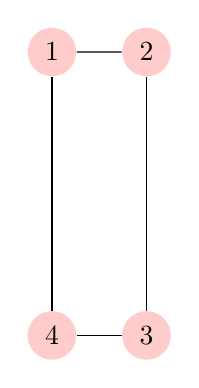
\begin{tikzpicture}
  [scale=.6,auto=left,every node/.style={circle,fill=red!20}]
  \node (n1) at (1,7) {1};
  \node (n2) at (3,7)  {2};
  \node (n4) at (1,1)  {4};
  \node (n3) at (3,1)  {3};

  \foreach \from/\to in {n1/n2,n2/n3,n3/n4,n1/n4}
    \draw (\from) -- (\to);

\end{tikzpicture}
\caption{ Example Graph}\label{17g1}
\end{center}
\end{figure}
\begin{figure}
\begin{center}
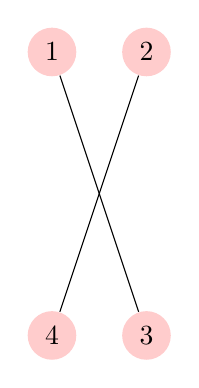
\begin{tikzpicture}
  [scale=.6,auto=left,every node/.style={circle,fill=red!20}]
  \node (n1) at (1,7) {1};
  \node (n2) at (3,7)  {2};
  \node (n4) at (1,1)  {4};
  \node (n3) at (3,1)  {3};

  \foreach \from/\to in {n1/n3,n2/n4}
    \draw (\from) -- (\to);

\end{tikzpicture}
\caption{ Complement of Graph \ref{17g1}}\label{17g2}
\end{center}
\end{figure}
\begin{figure}
\begin{center}
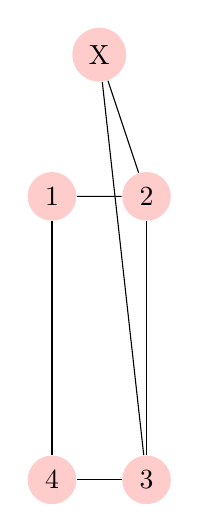
\begin{tikzpicture}
  [scale=.6,auto=left,every node/.style={circle,fill=red!20}]
  \node (n1) at (1,7) {1};
  \node (n2) at (3,7)  {2};
  \node (n4) at (1,1)  {4};
  \node (n3) at (3,1)  {3};
  \node (n5) at (2,10) {X};
  \foreach \from/\to in {n1/n2,n2/n3,n3/n4,n1/n4,n3/n5,n2/n5}
    \draw (\from) -- (\to);

\end{tikzpicture}
\caption{ Adding a vertex and adding edges from that vertex to some subset of vertices to the graph \ref{17g1}}\label{17g3}
\end{center}
\end{figure}

\begin{figure}
\begin{center}
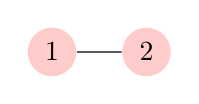
\begin{tikzpicture}
  [scale=.6,auto=left,every node/.style={circle,fill=red!20}]
  \node (n1) at (1,7) {1};
  \node (n2) at (3,7)  {2};

  \foreach \from/\to in {n1/n2}
    \draw (\from) -- (\to);

\end{tikzpicture}
\caption{ Example Graph $G_1$ for Cartesian Product}\label{17g4}
\end{center}
\end{figure}

\begin{figure}
\begin{center}
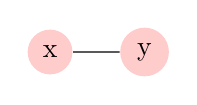
\begin{tikzpicture}
  [scale=.6,auto=left,every node/.style={circle,fill=red!20}]
  \node (n1) at (1,7) {x};
  \node (n2) at (3,7)  {y};

  \foreach \from/\to in {n1/n2}
    \draw (\from) -- (\to);

\end{tikzpicture}
\caption{ Example Graph $G_2$ for Cartesian Product}\label{17g5}
\end{center}
\end{figure}

\begin{figure}
\begin{center}
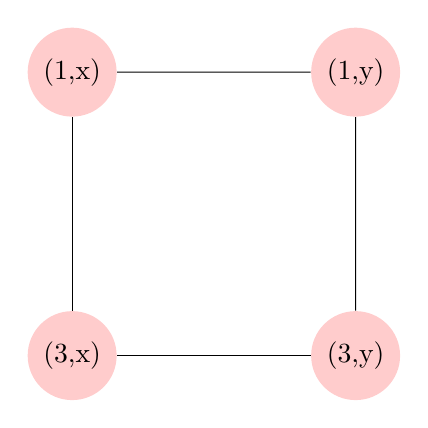
\begin{tikzpicture}
  [scale=.6,auto=left,every node/.style={circle,fill=red!20}]
  \node (n1) at (1,7) {(1,x)};
  \node (n2) at (7,7)  {(1,y)};
   \node (n3) at (1,1) {(3,x)};
   \node (n4) at (7,1) {(3,y)};
   
  \foreach \from/\to in {n1/n2,n1/n3,n2/n4,n3/n4}
    \draw (\from) -- (\to);

\end{tikzpicture}
\caption{ Cartesian Product $G_3$ of $G_1$ Figure \ref{17g4} and $G_2$ Figure \ref{17g5}}\label{17g6}
\end{center}
\end{figure}
\begin{figure}
\begin{center}

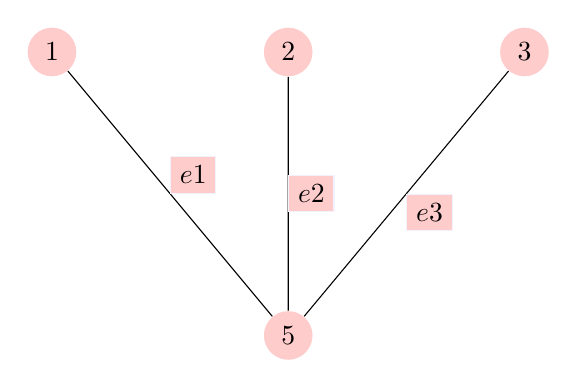
\begin{tikzpicture}
  [scale=.6,auto=left,every node/.style={circle,fill=red!20}]
  \tikzstyle{weight} = [draw=blue!5,shape=rectangle]
  \node (n1) at (-1,5) {1};
  \node (n2) at (4,5)  {2};
  \node (n3) at (9,5)  {3};
  \node (n4) at (4,-1) {5};
 
\foreach \source /\dest /\weight in {n1/n4/e1,n2/n4/e2,n3/n4/e3} 
   \draw (\source) --node[weight] {$\weight$}  (\dest);
 
  \end{tikzpicture}
\caption { A Graph for line graph example}\label {17g7}
\end{center}
\end{figure}

\begin{figure}
\begin{center}

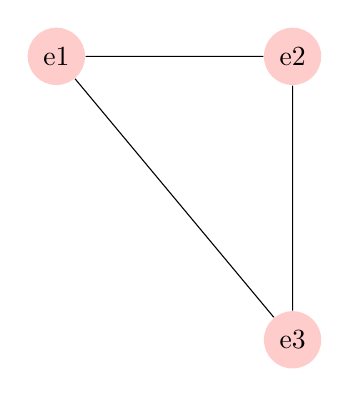
\begin{tikzpicture}
  [scale=.6,auto=left,every node/.style={circle,fill=red!20}]
  \tikzstyle{weight} = [draw=blue!5,shape=rectangle]
  \node (n1) at (-1,5) {e1};
  \node (n2) at (4,5)  {e2};
  \node (n3) at (4,-1) {e3};
 
\foreach \source /\dest  in {n1/n2,n2/n3,n3/n1} 
   \draw (\source) -- (\dest);
 
  \end{tikzpicture}
\caption { A Line Graph for a Graph in Figure \ref{17g7}}\label {17g8}
\end{center}
\end{figure}

Then Rishnak pointed out that Petersen Graph they had discussed earlier was the complement of the line graph of $K_5$. Ajur knew $K_5$ has 10 edges and Petersen graph has 10 edges and mentally verified that they matched. Ajur calculated that the line graph of $K_5$ is regular graph of degree 6 and hence its complement will be regular graph of degree 3 and that matched. But still he has to verify Rishnak's assertion. He decided to work on it later.

Rishnak realising that it was getting late, spent a few minutes But talking about Paul Erd\H{o}s and Renyi construction of a graph. In this method for a graph with $n$ vertices and $e$ edges, for every unordered pair of vertices  an edge is present with a probability of $\frac{e}{\frac{n \times (n-1)}{2}}$. Ajur needed time to digest all the material. So Ajur and Jura drifted away and Rishnak proceeded to meet his ghost friends.

Rishnak showed a graph generated by Erd\H{o}s Renyi model with 5 vertices 5 edges (so edge probability is 0.5  =$ \frac{5}{10}$) shown in Figure \ref {17g9} \footnote{Generated using Sage Math (CoCALC) \url{https://cocalc.com/}}
\begin{figure}
\begin{center}
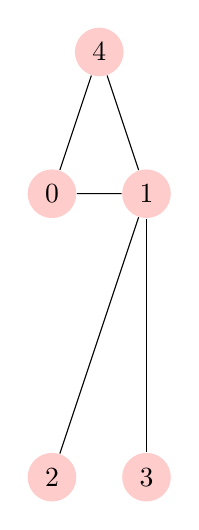
\begin{tikzpicture}
  [scale=.6,auto=left,every node/.style={circle,fill=red!20}]
  \node (n1) at (1,7) {0};
  \node (n2) at (3,7)  {1};
  \node (n4) at (1,1)  {2};
  \node (n3) at (3,1)  {3};
  \node (n5) at (2,10) {4};
  \foreach \from/\to in {n1/n5,n1/n2,n2/n5,n2/n4,n2/n3}
    \draw (\from) -- (\to);

\end{tikzpicture}
\caption{ Randomly Generated Graph using Erd\H{o}s Renyi Model with 5 vertices and 5 edges(so edge probability is 0.5  =$ \frac{5}{10}$)  }\label{17g9}
\end{center}
\end{figure}